%-------------------------------------------------------------------------
\section{Introduction}
Estimating surface normals from a noisy
point cloud benefits many applications in computer graphics, geometry
processing and reverse engineering. Accurate normal estimation allows a better reconstructing and rendering of point-based
surfaces \cite{DBLP:journals/cgf/OtireliGG09,DBLP:conf/siggraph/RusinkiewiczL00,WangGYTZ12,wangjun_cgf13}, anisotropic smoothing \cite{DBLP:journals/cagd/LangeP05} to name just a few.

With the assumption that the underlying surface is smooth everywhere, regression-based techniques \cite{DBLP:conf/siggraph/HoppeDDMS92,GuennebaudG07,CazalsP05,MitraNG04} use the whole neighborhoods to estimate normals. However, when a point is near sharp features, its neighborhood may be anisotropic and sampled from several piecewise surfaces.
In such case, all regression-based methods tend to smooth sharp features, since the normal estimation of the point may be influenced by its neighbors lying on some other surfaces.
%
To estimate normals more faithfully for point clouds with sharp features, Li \etal \cite{DBLP:journals/cg/LiSKCDJ10} (RNE) employed the robust statistics to classify points around sharp features into consistent sub-neighbors represented by different tangent planes.
%
However, this method is sensitive to the density variation, as shown in the bottom row of \fig \ref{fig:example}. Boulch \etal \cite{DBLP:journals/cgf/BoulchM12} (HF) introduced a uniform sampling strategy to overcome the influence of density variation.
%
However, the computed normals are unreliable for the points near sharp features, as shown in \fig \ref{fig:example}.
%
Moreover, this method tends to blur a sharp feature when the dihedral angel is large.
%
\begin{figure*}[htbp]
\begin{center}
    \begin{tabular}{c c c}
        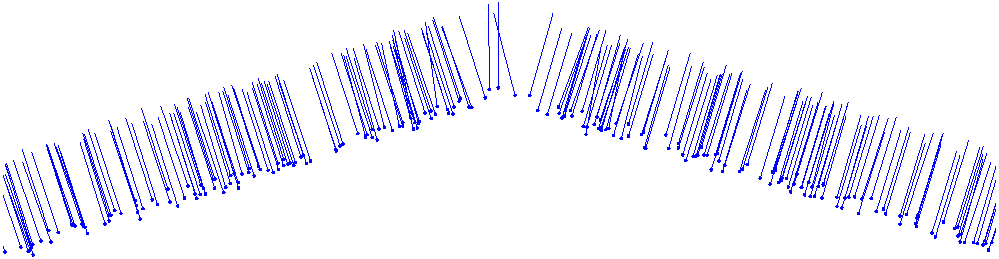
\includegraphics[width=0.3\linewidth]{example7_rne} &
        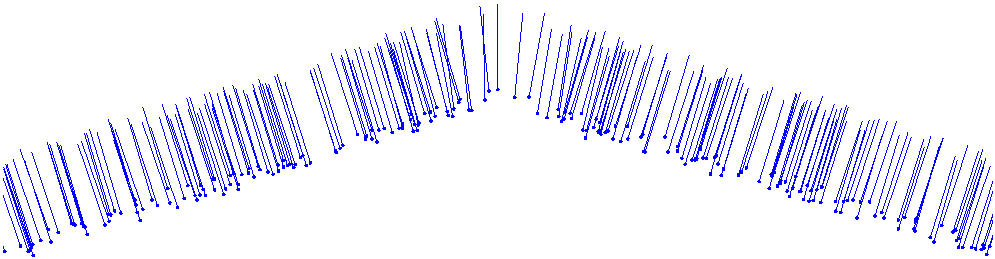
\includegraphics[width=0.3\linewidth]{example7_hf} &
        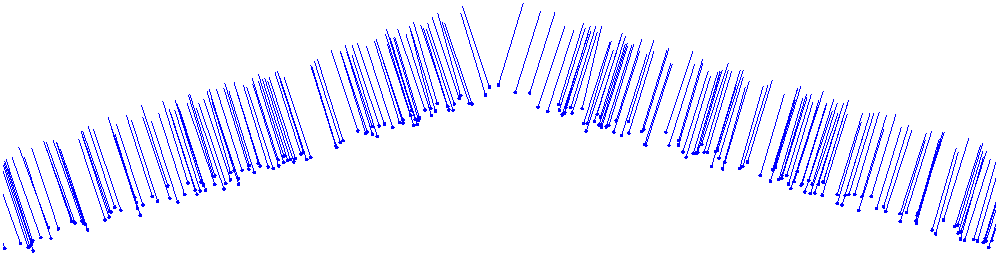
\includegraphics[width=0.3\linewidth]{example7_our}\\
        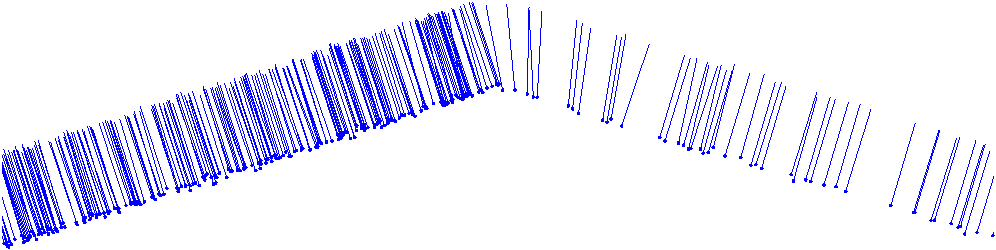
\includegraphics[width=0.3\linewidth]{example6_rne} &
        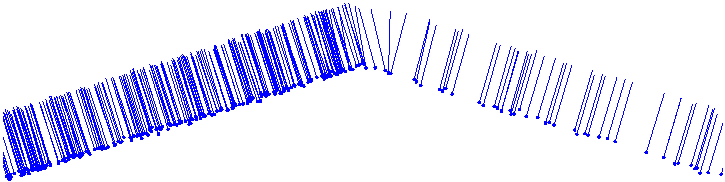
\includegraphics[width=0.3\linewidth]{example6_hf} &
        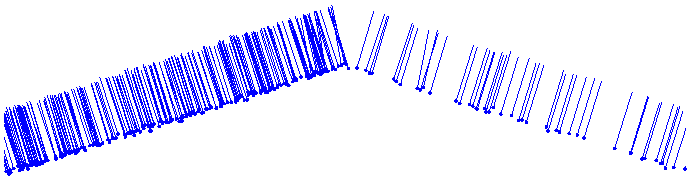
\includegraphics[width=0.3\linewidth]{example6_our}
    \end{tabular}
    \caption{\label{fig:example}
    Reconstructed normals of two plans with shallow angle by Li~\etal~\cite{DBLP:journals/cg/LiSKCDJ10} (left), Boulch~\etal~\cite{DBLP:journals/cgf/BoulchM12} (middle) and our algorithm (right). respectively.
    The points are sampled uniformly in the top row and non-uniformly in the bottom row.
    }
\end{center}
\end{figure*}

When a point is extremely near a sharp feature, it is hard to estimate its normal or classify its neighbors faithfully only by using the distance information.
%
To overcome this challenge, we present a novel robust approach to select a consistent neighborhood utilizing the structure of the underlying piecewise surfaces.
%
These surfaces can be approximated by planes and each of them is a 2D subspace, relative to the 3D Euclidean space where the model is embedded.
Thus, the segmentation of the neighborhood of a point can be solved as a subspace clustering problem, which has widespread applications in computer vision.
%
The Low-Rank Representation (LRR), emerging in machine learning, is a powerful tool in subspace clustering \cite{DBLP:journals/corr/abs-1010-2955,LiuLY10}.
It captures the global structure of the data robustly assuming that the subspaces are independent.
%
For our problem, the subspaces near sharp features are dependent, \ie the sum of the dimension of these subspaces is larger than three.
The standard low-rank method tends to fail for such case.
%
Hence we present a new low-rank subspace clustering framework with prior knowledge to handle more general subspace clustering.
In addition, we observe that the computation of normals which are not near sharp features (i.e. smooth regions) are reliable even with traditional regression-based methods, such as PCA.
%
Based on this observation, we design an unsupervised learning process to estimate the guidance from reliable regions. \re{Although it is relatively time-consuming, the consistent neighbors of a point can be effectively detected even in the presence of noise, which has many applications, including normal estimation and feature extraction,~\etc.} \fig~\ref{fig:flow_chart} gives the pipeline of our method.
The contributions of our work are summarized as follows:
\begin{itemize}
  \item The standard LRR model can only work under the assumption that the data are sampled from multiple independent subspaces. We provide a new low-rank subspace clustering framework with prior knowledge (LRSCPK) for more general subspace clustering. The prior knowledge can be obtained by many ways for different applications.
  %The standard LRR model can only work under the assumption that the data are sampled from multiple independent subspaces. By enforcing explicit structural constraint for the representation matrix, we provide a new method, named Structure Constrained LRR (SCLRR) for more general disjoint subspace clustering.
  \item For normal estimation, we use LRSCPK to segment and identify consistent subneighborhood and compute accurate normal from the subneighborhood.
      An unsupervised learning process is designed to estimate the prior knowledge from reliable regions, which are utilized in LRSCPK to classify unreliable regions close, even extremely close to sharp features.
       The estimated normals preserve sharp features even in the presence of noise and anisotropic samplings.

%  \item The sub-neighborhoods generated are useful in many applications, and we demonstrate how to use it for robust normal estimation and feature detection. I do not think the sub-neighborhood itself is useful. So the contributions should be completely re-written. I think there are two contributions: 1) the new subspace clustering method; 2) the feature-preserving normal estimation method.
\end{itemize}
%
